% !TEX root = saveliev_physics_general_course_1.tex
%!TEX TS-program = pdflatex
%!TEX encoding = UTF-8 Unicode


\chapter{NON-INERTIAL REFERENCE FRAMES}\label{chap:4}

\section{Forces of Inertia}\label{sec:4_1}

Newton's laws are obeyed only in inertial reference frames. A given body travels with the same acceleration a relative to all inertial frames. Any non-inertial reference frame travels with a certain acceleration relative to inertial frames, therefore the acceleration of a body in a non-inertial reference frame $\vec{a}'$ will differ from $\vec{a}$. Let us use the symbol $\vec{a}_0$ to denote the difference between the accelerations of a body in an inertial and a non-inertial reference frame:
\begin{equation}\label{eq:4_1}
\vec{a} - \vec{a}' = \vec{a}_0.
\end{equation}

\noindent
For a non-inertial frame in translational motion, $\vec{a}_0$ is the same for all points of space ($\vec{a}_0=\text{constant}$) and is the acceleration of the non-inertial reference frame. For a rotating non-inertial frame, $\vec{a}_0$ will be different at different points of space [$\vec{a}_0=\vec{a}_0(\vec{r}')$, where $\vec{r}'$ is the position vector determining the position of a point relative to the non-inertial reference frame].

Let the resultant of all the forces produced by the action of other bodies on the given body be $\vec{F}$. Hence, according to Newton's second law, the acceleration of the body relative to any inertial frame is
\begin{equation*}
\vec{a} = \frac{1}{m}\vec{F}.
\end{equation*}

\noindent
The acceleration of the body relative to a non-inertial frame, in accordance with \eqn{4_1}, can be represented in the form
\begin{equation*}
\vec{a}' = \vec{a} - \vec{a}_0 = \frac{1}{m}\vec{F} - \vec{a}_0.
\end{equation*}

\noindent
Hence, it follows that even when $\vec{F}=0$, the body will travel relative to the non-inertial reference frame with the acceleration---$\vec{a}_0$, \ie, as if a force equal to ---$m\vec{a}_0$ acted on it.

What has been said above signifies that we can use Newton's equations in describing motion in non-inertial reference frames, if in addition to the forces due to the action of bodies on one another, we take into account the so-called \textbf{forces of inertia} $\vec{F}_{\text{in}}$. The latter should be assumed equal to the product of the mass of a body and the difference between its accelerations relative to the inertial and non-inertial reference frames taken with the opposite sign:
\begin{equation}\label{eq:4_2}
\vec{F}_{\text{in}} = -m(\vec{a} - \vec{a}') = m\vec{a}_0.
\end{equation}

\begin{figure}[t]
	\begin{center}
		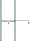
\includegraphics[scale=0.95]{figures/ch_04/fig_4_1.pdf}
		\caption[]{}
		\label{fig:4_1}
	\end{center}
\end{figure}

\noindent
The equation of Newton's second law for a non-inertial reference frame will accordingly be
\begin{equation}\label{eq:4_3}
m\vec{a}' = \vec{F} + \vec{F}_{\text{in}}.
\end{equation}

We shall explain our statement by the following example. Let us consider a cart with a bracket secured on it from which a ball is suspended on a string (\fig{4_1}). As long as the cart is at rest or is moving without acceleration, the string is vertical, and the force of gravity $\vec{P}$ is balanced by the reaction of the string $\vec{F}_{\text{r}}$. Now let us bring the cart into translational motion with the acceleration $\vec{a}_0$. The string will deviate from a vertical line through an angle such that the resultant of the forces $\vec{P}$ and $\vec{F}_{\text{r}}$ imparts an acceleration of $\vec{a}_0$ to the ball. The ball will be at rest relative to a reference frame associated with the cart, although the resultant of the forces $\vec{P}$ and $\vec{F}_{\text{r}}$ differs from zero. The absence of acceleration of the ball relative to this reference frame can be explained formally by the fact that in addition to the forces $\vec{P}$ and $\vec{F}_{\text{r}}$ whose sum equals $m\vec{a}_0$, the force of inertia $\vec{F}_{\text{in}}=-m\vec{a}_0$ also acts on the ball.

The introduction of inertial forces permits us to describe the motion of bodies in any (both inertial and non-inertial) reference frames using the same equations of motion.

One must understand distinctly that the forces of inertia may never be treated on a par with such forces as elastic, gravitational, and friction ones, \ie, with forces produced by the action on a body of other bodies. Forces of inertia are due to the properties of the reference frame in which mechanical phenomena are being considered. In this sense, they can be called fictitious forces.

The consideration of forces of inertia is not a necessity. Any motion, in principle, can always be considered relative to an inertial reference frame. In practice, however, it is exactly the motion of bodies relative to non-inertial reference frames, for instance, relative to the Earth's surface, that is often of interest to us. The use of inertial forces makes it possible to solve the relevant problem directly relative to such a reference frame, and this is frequently much simpler than consideration of the motion in an inertial frame.

\begin{figure}[t]
	\begin{center}
		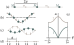
\includegraphics[scale=0.85]{figures/ch_04/fig_4_2.pdf}
		\caption[]{}
		\label{fig:4_2}
	\end{center}
\vspace{-0.2cm}
\end{figure}

A feature of inertial forces is that they are proportional to the mass of a body. Owing to this property, inertial forces are similar to gravitational ones. Imagine that we are in a closed cab removed from all external bodies and moving with the acceleration $\vec{g}$ in the direction which we shall call the ``top'' (\fig{4_2}). All the bodies in the cab will behave as if they experienced the force of inertia $-m\vec{g}$. In particular, a spring to whose end a body of mass $m$ is fastened will stretch so that the elastic force balances the force of inertia $m\vec{g}$. The same phenomena will be observed, however, when the cab is stationary and is near the Earth's surface. Having no possibility of ``looking out'' of the cab, we would not be able to establish by any experiments conducted in the cab whether the force $-m\vec{g}$ is due to its accelerated motion or to the action of the Earth's gravitational field. On these grounds, we speak of the equivalence of forces of inertia and gravitation. This equivalence underlies Albert Einstein's general theory of relativity.

\section{Centrifugal Force of Inertia}\label{sec:4_2}

Let us consider a disk rotating about a vertical axis $z'$ perpendicular to it with the angular velocity $\omega$ (\fig{4_3}). A ball fitted onto a spoke and connected to the centre of the disk by a spring rotates together with the disk. The ball occupies a position on the spoke such that the force $\vec{F}_{\text{spr}}$ stretching the spring is equal to the product of the mass of the ball $m$ and its acceleration $\vec{a}_n = -\omega^2R$ [see \eqn{1_102}; $\vec{R}$ is a position vector drawn to the ball from the centre of the disk. Its magnitude $R$ gives the distance from the centre of the disk to the ball]:
\begin{equation}\label{eq:4_4}
\vec{F}_{\text{spr}} = -m\omega^2\vec{R}.
\end{equation}

\begin{figure}[t]
	\begin{center}
		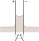
\includegraphics[scale=0.95]{figures/ch_04/fig_4_3.pdf}
		\caption[]{}
		\label{fig:4_3}
	\end{center}
\end{figure}

The ball is at rest relative to the reference frame associated with the disk. This can be formally explained by the circumstance that apart from the force~\eqref{eq:4_4}, the ball experiences the force of inertia
\begin{equation}\label{eq:4_5}
\vec{F}_{\text{cf}} = m\omega^2\vec{R}.
\end{equation}

\noindent
directed along a radius from the centre of the disk.

The force of inertia~\eqref{eq:4_5} set up in a rotating (relative to inertial frames) reference frame is called the centrifugal force of inertia. This force acts on a body in a rotating reference frame regardless of whether the body is at rest in this frame (as we have assumed up to now) or is moving relative to it with the velocity $\vec{v}'$.

If the position of a body in a rotating reference frame is characterized by the position vector $\vec{r}'$, then the centrifugal force of inertia can be represented in the form of a vector triple product
\begin{equation}\label{eq:4_6}
\vec{F}_{\text{cf}} = m [\vec{\omega} \times (\vec{r}'\times\vec{\omega})].
\end{equation}

\noindent
Indeed, the vector $\vec{b}=\vec{r}'\times\vec{\omega}$ is directed at right angles to the vectors $\vec{\omega}$ and $\vec{F}_{\text{cf}}$ ``toward us'' (\fig{4_4}), and its magnitude is $\omega r'\sin\alpha=\omega R$. The vector product of the mutually perpendicular vectors $m\vec{\omega}$ and $\vec{b}$ coincides in direction with $\vec{F}_{\text{cf}}$, and its magnitude is $m\omega b=m\omega^2R=\vec{F}_{\text{cf}}$.

\begin{figure}[t]
	\begin{center}
		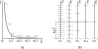
\includegraphics[scale=1]{figures/ch_04/fig_4_4.pdf}
		\caption[]{}
		\label{fig:4_4}
	\end{center}
\end{figure}

In the accurate solution of problems on the motion of bodies relative to the Earth's surface, account must be taken of the centrifugal force of inertia equal to $m\omega^2R$, where $m$ is the mass of a body, $\omega$ is the angular velocity of the Earth in its rotation about its axis, and $R$ is the distance to the body from the Earth's axis (\fig{4_5}). When the height of bodies above the Earth's surface (their altitude) is not great, we may assume that $R=R_{\text{E}}\cos\varphi$ ($R_{\text{E}}$ is the Earth's radius, and $\varphi$ is the latitude of the locality). The expression for the centrifugal force of inertia thus becomes
\begin{equation}\label{eq:4_7}
F_{\text{cf}} = m\omega^2 R_{\text{E}}\cos\varphi.
\end{equation}

\begin{figure}[t]
	\begin{center}
		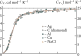
\includegraphics[scale=1]{figures/ch_04/fig_4_5.pdf}
		\caption[]{}
		\label{fig:4_5}
	\end{center}
	\vspace{-0.8cm}
\end{figure}

The acceleration of free fall of bodies $\vec{g}$ observed relative to the Earth is due to the action of the force $\vec{F}_{\text{g}}$ with which a body is attracted by the Earth, and of the force $\vec{F}_{\text{cf}}$. The resultant of these forces
\begin{equation}\label{eq:4_8}
\vec{P} = \vec{F}_{\text{g}} + \vec{F}_{\text{cf}}
\end{equation}

\noindent
is the force of gravity equal to $m\vec{g}$ [see \eqn{2_38}].

The difference between the force of gravity $\vec{P}$ and the force of attraction to the Earth $\vec{F}_{\text{g}}$ is not great because the centrifugal force of inertia is much smaller than $\vec{F}_{\text{g}}$. Thus, for a mass of \SI{1}{\kilo\gram}, the maximum value of $F_{\text{cf}}$ observed at the equator is
\begin{equation*}
m\omega^2 R_{\text{E}} = 1 \times \left(\frac{2\pi}{86400}\right)^2 \times \num{6.4e6} = \SI{0.035}{\newton}
\end{equation*}

\noindent
whereas $\vec{F}_{\text{g}}$ approximately equals \SI{9.8}{\newton}, \ie, is almost $300$ times greater.

The angle $\alpha$ between the directions of $\vec{F}_{\text{g}}$ and $\vec{P}$ (see \fig{4_5}) can be found by using the theorem of sines:
\begin{equation*}
\frac{\sin\alpha}{\sin\varphi} = \frac{F_{\text{g}}}{P} = \frac{m\omega^2 R_{\text{E}}\cos\varphi}{mg} \approx \frac{\SI{0.035}{\newton}}{\SI{9.8}{\newton}} \cos\varphi \approx 0.0035 \cos\varphi
\end{equation*}

\noindent
whence
\begin{equation*}
\sin\alpha \approx 0.0035\sin\varphi\cos\varphi \approx 0.0018 \sin 2\varphi.
\end{equation*}

\noindent
The sine of a small angle may be approximately replaced by the value of the angle itself. Such approximation yields
\begin{equation}\label{eq:4_9}
\alpha \approx 0.0018 \sin 2\varphi.
\end{equation}

\noindent
Thus, the angle $\alpha$ varies within the limits from zero (at the equator, where $\varphi=0$, and at the poles, where $\varphi=\SI{90}{\degree}$) to \SI{0.0018}{\radian} or $6'$ (at a latitude of \SI{45}{\degree}).

The direction of the force $\vec{P}$ coincides with that of a string tensioned by a weight, which is called the direction of a plumb or the vertical direction. The force $\vec{F}_{\text{g}}$ is directed toward the centre of the Earth. Therefore, a vertical line is directed toward the centre of the Earth only at the poles and the equator, and deviates at intermediate latitudes by the angle $\alpha$ determined by expression~\eqref{eq:4_9}.

The difference $F_{\text{g}}-P$ vanishes at the poles and reaches a maximum equalling $0.3$\% of the force $F_{\text{g}}$ at the equator. Owing to the oblateness of the Earth, the force $F_{\text{g}}$ varies somewhat with the latitude, being about $0.2$\% less at the equator than at the poles. As a result, the acceleration of free fall varies with the latitude within the limits from \SI{9.780}{\metre\per\square\second} at the equator to \SI{9.832}{\metre\per\square\second} at the poles. The value of $g=\SI{9.80665}{\metre\per\square\second}$ is taken as the standard one.

We must note that a freely falling body moves relative to an inertial, for example, a heliocentric, reference frame with the acceleration $\vec{a}=\vec{F}_{\text{g}}/m$ (and not $\vec{g}$). A glance at \fig{4_5} shows that from the equality of the acceleration $g$ for different bodies we get the equality of the accelerations $a$. Indeed, the triangles constructed on the vectors $\vec{F}_{\text{g}}$ and $\vec{P}$ for different bodies are similar (the angles $\alpha$ and $\varphi$ for all bodies at the given point on the Earth's surface are identical). Consequently, the ratio $F_{\text{g}}/P$, which coincides with the ratio $a/g$ is the same for all the bodies. Hence, it follows that we get identical values of $a$ for the same $g$'s.

\section{Coriolis Force}\label{sec:4_3}

When a body moves relative to a rotating reference frame, another force called the \textbf{Coriolis force} appears in addition to the centrifugal force of inertia.

The appearance of a Coriolis force can be detected in the following experiment. Let us take a horizontally arranged disk that can rotate about a vertical axis. We draw radial line $O$A on the disk (\fig{4_6}a). Let us launch a ball with the velocity $\vec{v}'$ in the direction from $0$ to A. If the disk does not rotate, the ball will roll along the radius we have drawn. If the disk is rotated in the direction shown by the arrow, however, then the ball will roll along dash curve $0$B, and its velocity relative to the disk $\vec{v}'$ will change its direction. Consequently, the ball behaves relative to the rotating reference frame as if it experiences the force $\vec{F}_{\text{Cor}}$ perpendicular to the velocity $\vec{v}'$.

\begin{figure}[t]
	\begin{center}
		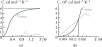
\includegraphics[scale=1]{figures/ch_04/fig_4_6.pdf}
		\caption[]{}
		\label{fig:4_6}
	\end{center}
	\vspace{-0.8cm}
\end{figure}

To make the ball roll on the rotating disk along the radius, we must install a guide, for instance, in the form of rib $0$A (\fig{4_6}b). When the ball is rolling, the guide rib exerts the force $\vec{F}_{\text{rib}}$ on it. The ball travels with a velocity constant in direction relative to the rotating frame (disk). This can formally be explained by the fact that the force $\vec{F}_{\text{rib}}$ is balanced by the force of inertia $\vec{F}_{\text{Cor}}$ applied to the ball at right angles to the velocity $\vec{v}'$. It is exactly the force $\vec{F}_{\text{Cor}}$ that is the Coriolis force.

Let us first find an expression for the Coriolis force in the particular case when a particle $m$ moves relative to a rotating reference frame uniformly along a circle in a plane perpendicular to the axis of rotation with its centre on this axis (\fig{4_7}). Let $\vec{v}'$ stand for the velocity of the particle relative to the rotating frame. The velocity $\vec{v}$ of the particle relative to a fixed (inertial) reference frame has the magnitude $v'+\omega R$ in case (a) and $|v-\omega R|$ in case (b), where $\omega$ is the angular velocity of the rotating frame, and $R$ is the radius of the circle (see \eqn{1_99}].

\begin{figure}[t]
	\begin{center}
		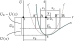
\includegraphics[scale=1]{figures/ch_04/fig_4_7.pdf}
		\caption[]{}
		\label{fig:4_7}
	\end{center}
	\vspace{-0.8cm}
\end{figure}

For the particle to move relative to the fixed frame along a circle with the velocity $v=v'+\omega R$, it must experience the force $\vec{F}$ directed  toward the centre of the circle, for example, the force of tension of the string by means of which the particle is tied to the centre of the circle (see \fig{4_7}a). The magnitude of this force is
\begin{equation}\label{eq:4_10}
F = m a_{\hatvec{n}} = \frac{mv^2}{R} = \frac{m(v'+\omega R)^2}{R} = \frac{mv'^2}{R} + 2mv'\omega + m\omega^2 R.
\end{equation}

\noindent
The particle in this case moves relative to the rotating frame with the acceleration $a_{\hatvec{n}}'=v'^2/R$, \ie, as if it experienced the force
\begin{equation}\label{eq:4_11}
m a_{\hatvec{n}}' = \frac{mv^2}{R} = F - 2mv'\omega - m\omega^2 R
\end{equation}

\noindent
[see \eqn{4_10}]. Thus, the particle behaves in the rotating frame as if two other forces directed away from the centre acted on it in addition to the force $\vec{F}$ directed toward the centre. These two forces are $\vec{F}_{\text{cf}}=m\omega^2 R$ and $\vec{F}_{\text{Cor}}$ whose magnitude equals $2mv'\omega$ (\fig{4_7}a). It is easy to see that the force $\vec{F}_{\text{Cor}}$ can be represented in the form
\begin{equation}\label{eq:4_12}
\vec{F}_{\text{Cor}} = 2m(\vec{v}'\times\vec{\omega}).
\end{equation}

\noindent
The force~\eqref{eq:4_12} is exactly the Coriolis force. This force vanishes when $\vec{v}'=0$. The force $\vec{F}_{\text{cf}}$ does not depend on $\vec{v}'$---as we have already noted, it acts both on bodies at rest and on moving ones.

For the case shown in \fig{4_7}b, we have
\begin{equation*}
	F = \frac{mv^2}{R} = \frac{m(v'-\omega R)^2}{R} = \frac{mv'^2}{R} - 2mv'\omega + m\omega^2 R.
\end{equation*}

\noindent
Accordingly,
\begin{equation*}
\frac{mv'^2}{R} = F + 2mv'\omega - m\omega^2 R.
\end{equation*}

\noindent
Consequently, in a rotating frame, the particle behaves as if it experienced two forces $\vec{F}$ and $\vec{F}_{\text{Cor}}$ directed toward the centre of the circle, and also the force $\vec{F}_{\text{cf}}=m\omega^2R$ directed away from the centre (see \fig{4_7}b). The force $\vec{F}_{\text{Cor}}$ in this case can be represented in the form of \eqn{4_12}.

\begin{figure}[t]
	\begin{center}
		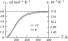
\includegraphics[scale=1]{figures/ch_04/fig_4_8.pdf}
		\caption[]{}
		\label{fig:4_8}
	\end{center}
	\vspace{-0.8cm}
\end{figure}

Now let us pass over to finding an expression for the Coriolis force when a particle moves arbitrarily relative to a rotating reference frame. Let us associate the coordinate axes $x', y', z'$ with the rotating frame, and make the axis $z'$ coincide with the axis of rotation (\fig{4_8}). The position vector of the particle can therefore be represented in the form
\begin{equation}\label{eq:4_13}
\vec{r}' = x'\vecuni{x}' + y'\vecuni{y}' + z'\vecuni{z}'
\end{equation}

\noindent
where $\vecuni{x}'$, $\vecuni{y}'$ and $\vecuni{z}'$ are the unit vectors of the coordinate axes. The unit vectors $\vecuni{x}'$ and $\vecuni{y}'$ rotate together with the reference frame with the angular velocity $\omega$, whereas the unit vector $\vecuni{z}'$ remains stationary.

The position of the particle relative to the fixed frame should be determined with the aid of the position vector $\vec{r}$. The symbols $\vec{r}'$ and $\vec{r}$, however, signify the same vector drawn from the origin of coordinates to the particle. An observer ``living'' in the rotating reference frame denoted this vector by $\vec{r}'$. According to his observations, the unit vectors $\vecuni{x}'$, $\vecuni{y}'$ and $\vecuni{z}'$ are stationary, therefore when differentiating \eqn{4_13}, he treats these unit vectors as if they are constants. A stationary observer uses the symbol $\vec{r}$. For him, the unit vectors $\vecuni{x}'$ and $\vecuni{y}'$ rotate with the velocity $\omega$ (the unit vector $\vecuni{z}'$ is stationary). Therefore, when differentiating the expression~\eqref{eq:4_13} equal to $\vec{r}$, he must treat $\vecuni{x}'$ and $\vecuni{y}'$ as functions of $t$ whose derivatives are
\begin{equation}\label{eq:4_14}
\dot{\hatvec{e}}_x' = \omega\vecuni{y}',\quad \dot{\hatvec{e}}_y' = -\omega\vecuni{x}'
\end{equation}

\noindent
[see \fig{4_8} and \eqn{1_56}; the unit vector $\vecuni{\perp x'}$ perpendicular to $\vecuni{x}'$ equals $\vecuni{y}'$ and the unit vector $\vecuni{\perp y'}$ perpendicular to $\vecuni{y'}$ equals $-\vecuni{x'}$]. For the second time derivatives of the unit vectors, we get
\begin{equation}\label{eq:4_15}
\ddot{\hatvec{e}}_x' = \omega\dot{\hatvec{e}}_y' = -\omega^2\vecuni{x}',\quad \ddot{\hatvec{e}}_y' = \omega\dot{\hatvec{e}}_x' = -\omega^2\vecuni{y}'.
\end{equation}

Let us find the velocity of the particle relative to the rotating reference frame. To do this, we differentiate the position vector~\eqref{eq:4_13} with respect to time, considering the unit vectors as constants:
\begin{equation}\label{eq:4_16}
\vec{v}' = \dot{\vec{r}}' = \dot{x}'\vecuni{x}' + \dot{y}'\vecuni{y}' + \dot{z}'\vecuni{z}'
\end{equation}

\noindent
If we now differentiate this expression, we get the acceleration of the particle relative to the rotating reference frame:
\begin{equation}\label{eq:4_17}
\vec{a}' = \dot{\vec{v}}' = \ddot{\vec{r}}' = \ddot{x}'\vecuni{x}' + \ddot{y}'\vecuni{y}' + \ddot{z}'\vecuni{z}'.
\end{equation}

Now we shall find the velocity of the particle relative to the fixed reference frame. For this purpose, we shall differentiate the position vector~\eqref{eq:4_13} ``from the positions'' of the stationary observer. Using the symbol $\vec{r}$ instead of $\vec{r}'$ (recall that $\vec{r}=\vec{r}'$), we get
\begin{equation}\label{eq:4_18}
\vec{v} = \dot{\vec{r}} = \dot{x}'\vecuni{x}' + x'\dot{\hatvec{e}}_x' + \dot{y}'\vecuni{y}' + y'\dot{\hatvec{e}}_y' + \dot{z}'\vecuni{z}' + z'\dot{\hatvec{e}}_z'.
\end{equation}

\noindent
Differentiating this expression with respect to $t$, we find the acceleration of the particle relative to the fixed frame:
\begin{equation*}
\vec{a} = \dot{\vec{v}} =
\ddot{x}'\vecuni{x}' + 2\dot{x}'\dot{\hatvec{e}}_x' + x'\ddot{\hatvec{e}}_y' + \ddot{y}'\vecuni{y}' + 2\dot{y}'\dot{\hatvec{e}}_y' + y'\ddot{\hatvec{e}}_y' + \ddot{z}'\vecuni{z}' + 2\dot{z}'\dot{\hatvec{e}}_z' + z'\ddot{\hatvec{e}}_z'.
\end{equation*}

\noindent
Taking into account Eqs.~\eqref{eq:4_14}, \eqref{eq:4_15}, and \eqref{eq:4_17}, we can transform the above expression into the form:
\begin{equation}\label{eq:4_19}
\vec{a} = \vec{a}' + 2\omega(\dot{x}'\vecuni{y}' - \dot{y}\vecuni{x}') - \omega^2(x'\vecuni{x}' + \dot{y}\vecuni{y}').
\end{equation}

Let us consider the vector product $\vecprod{\omega}{v}'$. We shall represent it in the form of a determinant [see \eqn{1_33}]:
\begin{equation}\label{eq:4_20}
\vecprod{\omega}{v}' = \begin{vmatrix}
\vecuni{x}' & \vecuni{y}' & \vecuni{z}'\\
\omega_x & \omega_y & \omega_z\\
v_x' & v_y' & v_z'
\end{vmatrix}.
\end{equation}

\noindent
According to \eqn{4_16}, $v_x=\dot{x}', v_y=\dot{y}', v_z=\dot{z}'$. In addition, for the direction of the coordinate axes that we have selected, we have $\omega_x=\omega_y=0, \omega_z=\omega$. Introduction of these values into \eqn{4_20} yields
\begin{equation}\label{eq:4_21}
\vecprod{\omega}{v}' = \begin{vmatrix}
\vecuni{x}' & \vecuni{y}' & \vecuni{z}'\\
0 & 0 & \omega\\
\dot{x}' & \dot{y}' & \dot{z}'
\end{vmatrix} = -\vecuni{x}'\omega\dot{y}' + \vecuni{y}'\omega\dot{x}'.
\end{equation}

\noindent
The result obtained shows that the second term of \eqn{4_19} can be written in the form $2\vecprod{\omega}{v}'$. The expression in parentheses in the last term of \eqn{4_19} equals the component of the position vector $\vec{r}'$ perpendicular to the axis of rotation (to the axis $z'$) [see \eqn{4_13}]. Let us denote this component by the symbol $\vec{R}$ (compare with \fig{1_33}). In view of everything said above, \eqn{4_19} can be written as follows:
\vspace{-12pt}
\begin{equation}\label{eq:4_22}
\vec{a} = \vec{a}' + 2\vecprod{\omega}{v}' - \omega^2\vec{R}.
\end{equation}

It follows from \eqn{4_22} that the acceleration of the particle relative to the fixed reference frame can be represented in the form of the sum of three accelerations: that relative to the rotating frame $\vec{a}'$, the acceleration equal to $-\omega^2\vec{R}$\footnote{The acceleration $\vec{a}_{\text{tr}}=-\omega^2\vec{R}$ is called transferable. It is the acceleration which a particle would have being at rest in a moving (in our case in a rotating) reference frame.}, and the acceleration
\begin{equation}\label{eq:4_23}
\vec{a}_{\text{Cor}} = 2\vecprod{\omega}{v}'
\end{equation}

\noindent
called the \textbf{Coriolis acceleration}.

For a particle to move with the acceleration~\eqref{eq:4_22}, bodies must act on it with the resultant force $\vec{F}=m\vec{a}$. According to \eqn{4_22}
\begin{equation}\label{eq:4_24}
m\vec{a}' = m\vec{a} - 2m\vecprod{\omega}{v}' + m\omega^2\vec{R} = \vec{F} + 2m\vec{v}'\times\vec{\omega} + m\omega^2\vec{R}
\end{equation}

\noindent
(transposition of the multipliers changes the sign of the vector product). The result obtained signifies that when compiling an equation of Newton's second law for a rotating reference frame, in addition to the forces of interaction account must be taken of the centrifugal force of inertia determined by \eqn{4_25}, and also of the Coriolis force which even in the most general case is determined by \eqn{4_12}. We must note that the Coriolis force is always in a plane perpendicular to the axis of rotation.

It follows from a comparison of Eqs.~\eqref{eq:4_14}, \eqref{eq:4_16}, and \eqref{eq:4_18} that
\begin{equation*}
\vec{v} = \vec{v}' + x'\dot{\hatvec{e}}_x' + y'\dot{\hatvec{e}}_y' = \vec{v}' + \omega(x'\vecuni{y}' - y'\vecuni{x}').
\end{equation*}

\noindent
Calculations similar to those which led us to \eqn{4_22} can help us see that the last term of the above expression equals $\vecprod{\omega}{v}'$. Hence,
\begin{equation}\label{eq:4_25}
\vec{v} = \vec{v}' + \vecprod{\omega}{v}'.
\end{equation}

\noindent
When $\vec{v}'=0$, this equation transforms into \eqn{1_100}.

%\begin{figure}[t]
%	\begin{minipage}[t]{0.35\linewidth}
%		\begin{center}
%			\includegraphics[scale=0.84]{figures/ch_04/fig_4_9.pdf}
%			\caption[]{}
%			\label{fig:4_9}
%		\end{center}
%	\end{minipage}
%	\hspace{-0.05cm}
%	\begin{minipage}[t]{0.35\linewidth}
%		\begin{center}
%			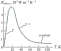
\includegraphics[scale=0.87]{figures/ch_04/fig_4_10.pdf}
%			\caption[]{}
%			\label{fig:4_10}
%		\end{center}
%	\end{minipage}
%	\hspace{-0.2cm}
%	\begin{minipage}[t]{0.3\linewidth}
%		\begin{center}
%			\includegraphics[scale=0.85]{figures/ch_04/fig_4_11.pdf}
%			\caption[]{}
%			\label{fig:4_11}
%		\end{center}
%	\end{minipage}
%\end{figure}
\begin{figure}[t]
	\begin{minipage}[t]{0.5\linewidth}
		\begin{center}
			\includegraphics[scale=1]{figures/ch_04/fig_4_9.pdf}
			\caption[]{}
			\label{fig:4_9}
		\end{center}
	\end{minipage}
	\hspace{-0.05cm}
	\begin{minipage}[t]{0.5\linewidth}
		\begin{center}
			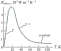
\includegraphics[scale=1.03]{figures/ch_04/fig_4_10.pdf}
			\caption[]{}
			\label{fig:4_10}
		\end{center}
	\end{minipage}
	\vspace{-0.4cm}
\end{figure}

\textbf{Examples of Motions in Which the Coriolis Force Manifests Itself.} In interpreting phenomena associated with the motion of bodies relative to the Earth's surface, it is sometimes necessary to take account of the influence of Coriolis forces. For example, in the free fall of bodies, a Coriolis force acts on them that causes them to deviate to the East from a vertical line (\fig{4_9}). This force is the greatest at the equator and vanishes at the poles.

A flying projectile also experiences deviations due to Coriolis forces (\fig{4_10}). When a projectile is fired from a gun facing North, it will deviate to the East in the northern hemisphere and to the West in the southern one. If a projectile is fired along a meridian to the South, the deviations will be the reverse. If a projectile is fired along the equator, Coriolis forces will press it toward the Earth if the shot was directed to the West, and lift it if the shot was directed to the East. We invite our reader to convince himself that the Coriolis force acting on a body moving along a meridian in any direction (to the North or South) has a rightward direction relative to that of motion in the northern hemisphere and a leftward one in the southern hemisphere. This is why rivers always wash out their right banks in the northern hemisphere and their left banks in the southern one. This is also why the rails of a double-track railway wear differently.

The Coriolis forces also manifest themselves in the oscillations of a pendulum. Figure~\ref{fig:4_11} shows the trajectory of a pendulum bob (it is assumed for simplicity's sake that the pendulum is at a pole). At the north pole, the Coriolis force will constantly be directed to the right in the direction of the pendulum's motion, and at the south pole to the left. As a result, the trajectory has the shape of a rosette.

As can be seen from the figure, the plane of oscillations of the pendulum turns clockwise relative to the Earth, and it completes one revolution a day. Relative to a heliocentric reference frame, the plane of oscillations remains unchanged, while the Earth rotates completing one revolution a day. It can be shown that at the latitude $\varphi$ the plane of oscillations of a pendulum turns through the angle of $2\pi\sin\varphi$ in a day.

Thus, observations of the rotation of the plane in which a pendulum oscillates (pendulums intended for this purpose are called Foucault pendulums) provide a direct proof of the Earth's rotation about its axis.

\section{Laws of Conservation in Non-Inertial Reference Frames}\label{sec:4_4}

The equations of motion in a non-inertial frame do not differ in any way from those of motion in an inertial reference frame when the forces of inertia are taken into account. Therefore, all the corollaries following from the equations of motion, particularly Eqs.~\eqref{eq:3_77}, \eqref{eq:3_88}, and \eqref{eq:3_118}, also hold in non-inertial reference frames.

\begin{figure}[t]
	\begin{minipage}[t]{0.5\linewidth}
		\begin{center}
			\includegraphics[scale=0.95]{figures/ch_04/fig_4_11.pdf}
			\caption[]{}
			\label{fig:4_11}
		\end{center}
	\end{minipage}
	\hspace{-0.05cm}
	\begin{minipage}[t]{0.5\linewidth}
		\begin{center}
			\includegraphics[scale=0.95]{figures/ch_04/fig_4_12.pdf}
			\caption[]{}
			\label{fig:4_12}
		\end{center}
	\end{minipage}
	\vspace{-0.45cm}
\end{figure}

Equation~\eqref{eq:3_77} acquires the following form for a non-inertial frame:
\begin{equation}\label{eq:4_26}
E_2-E_1 = A_{12,\text{non-cons}} + A_{12,\text{in}}
\end{equation}

\noindent
where $A_{12,\text{in}}$ is the work done by the forces of inertia.

Equations~\eqref{eq:3_88} and ~\eqref{eq:3_118} can be written as follows for a non-inertial frame:
\begin{align}
\diff{\vec{p}}{t} &= \sum\vec{F}_{\text{ext}} + \sum\vec{F}_{\text{in}}\label{eq:4_27}\\
\diff{\vec{L}}{t} &= \sum\vec{M}_{\text{ext}} + \sum\vec{M}_{\text{in}}\label{eq:4_28}.
\end{align}

Here $\vec{F}_{\text{ext}}$ is the force due to interaction, $\vec{F}_{\text{in}}$ is the force of inertia, $\vec{M}_{\text{ext}}$ and $\vec{M}_{\text{in}}$ are the moments of the above forces.

The centrifugal force of inertia $\vec{F}_{\text{cf}}=m\omega^2 R$ is conservative. Indeed, the work of this force is
\begin{equation*}
A_{12,\text{cf}} = \int_1^2\vec{F}_{\text{cf}}\,\deriv{\vec{r}} = m\omega^2\int_{1}^{2}\vec{R}\,\deriv{\vec{r}}.
\end{equation*}

\noindent
Inspection of \fig{4_12} shows that the projection of the vector $\deriv{\vec{r}}$ on the direction of the vector $\vec{R}$ equals $\deriv{R}$---the increment of the magnitude of $\vec{R}$. Consequently, $\vec{R}\deriv{\vec{r}}=R\,\deriv{R} = \deriv{R^2/2}$. Thus,
\begin{equation}\label{eq:4_29}
A_{12,\text{cf}} = m\omega^2 \int_{1}^{2} \deriv{R^2/2} = m\omega^2 \frac{R^2_2}{2} - m\omega^2 \frac{R^2_1}{2}.
\end{equation}

\noindent
The expression obtained does not obviously depend on the path along which the displacement from point $1$ to point $2$ occurred.

The conservative nature of the force $\vec{F}_{\text{cf}}$ makes it possible to introduce the potential energy of a particle $E_{\text{p,cf}}$ (the centrifugal energy) whose decrement determines the work of the centrifugal force of inertia:
\begin{equation}\label{eq:4_30}
A_{12,\text{cf}} = E_{\text{p,cf},1} - E_{\text{p,cf},2}
\end{equation}

\noindent
[see \eqn{3_30}]. A comparison of Eqs.~\eqref{eq:4_29} and \eqref{eq:4_30} shows that $E_{\text{p,cf}}=-m\omega^2R^2/2 + \text{constant}$. We may assume that the constant equals zero. We thus get the following expression for the centrifugal energy:
\begin{equation}\label{eq:4_31}
E_{\text{p,cf}} = -\frac{1}{2} m \omega^2 R^2.
\end{equation}

If we add \eqn{4_31} to the potential energy of a particle, then the work of the centrifugal force of inertia must not be included in the quantity $A_{12,\text{in}}$ in \eqn{4_26}.
